\documentclass[conference]{IEEEtran}
\IEEEoverridecommandlockouts
\usepackage{cite}
\usepackage{amsmath,amssymb,amsfonts}
\usepackage{algorithmic}
\usepackage{graphicx}
\usepackage{textcomp}
\usepackage{xcolor}
\usepackage{float}
\usepackage{tabularx}
\def\BibTeX{{\rm B\kern-.05em{\sc i\kern-.025em b}\kern-.08em
    T\kern-.1667em\lower.7ex\hbox{E}\kern-.125emX}}
\begin{document}

\title{Application of Machine Learning K-Means Clustering and Linear Regression in Determining the Risk Level of Pulmonary Tuberculosis}

\author{\IEEEauthorblockN{1\textsuperscript{st} Abhijit Pathak}
\IEEEauthorblockA{\textit{Assistant Professor} \\
\textit{BGC Trust University Bangladesh}\\
Chattogram, Bangladesh \\
abhijitpathak@bgctub.ac.bd \\
0000-0001-7734-0271}
\and
\IEEEauthorblockN{2\textsuperscript{nd} Ziaul Islam Bablu}
\IEEEauthorblockA{\textit{Research Assistant} \\
\textit{BGC Trust University Bangladesh}\\
Chattogram, Bangladesh \\
ziaulislambablu2@gmail.com \\
0009-0000-8783-8022}
\and
\IEEEauthorblockN{3\textsuperscript{rd} Towhidul Haque Limon}
\IEEEauthorblockA{\textit{Research Assistant} \\
\textit{BGC Trust University Bangladesh}\\
Chattogram, Bangladesh \\
towhidulhaque4455@gmail.com\\
0009-0002-4177-6991}
\and
\IEEEauthorblockN{4\textsuperscript{th} Sowmik Barua}
\IEEEauthorblockA{\textit{Research Assistant} \\
\textit{BGC Trust University Bangladesh}\\
Chattogram, Bangladesh \\
sowmikbarua7878@gmail.com \\
0009-0004-4974-3478}
\and
\IEEEauthorblockN{5\textsuperscript{th} Piyal Dey}
\IEEEauthorblockA{\textit{Research Assistant} \\
\textit{BGC Trust University Bangladesh}\\
Chattogram, Bangladesh \\
piyaldey6@gmail.com \\
0009-0000-8385-1617}
\and
\IEEEauthorblockN{6\textsuperscript{th} Mowmita Tajnin Jiba}
\IEEEauthorblockA{\textit{Research Assistant} \\
\textit{BGC Trust University Bangladesh}\\
Chattogram, Bangladesh \\
mowmitatajninj@gmail.com \\
0009-0000-7578-4813}
\and
\IEEEauthorblockN{7\textsuperscript{th} Touhidul Alam Seyam}
\IEEEauthorblockA{\textit{Research Assistant} \\
\textit{BGC Trust University Bangladesh}\\
Chattogram, Bangladesh \\
touhidulalam@bgctub.ac.bd \\
0009-0007-7512-1893}
}

\maketitle

\begin{abstract}
    Pulmonary tuberculosis (TB) remains a significant public health concern in densely populated regions like Bireuen, Bangladesh, which reported 755 cases in 2019 among a population of 400,000. This study used data from Bangabandhu Sheikh Mujib Medical University Hospital and the Health Department across 17 districts to identify high-risk areas and predict disease incidence. Utilizing K-Means clustering and Cluster-wise Regression, the analysis identified two high-risk areas in Cluster 1, six in Cluster 2, and nine in Cluster 3, with a regression analysis R-squared value of 0.5740, indicating moderate predictive capacity. These findings provide critical insights for public health authorities to devise targeted interventions and allocate resources effectively. Strategies such as targeted screening programs and improved access to diagnostic and treatment facilities in high-risk areas can help mitigate TB's impact. The study emphasizes the importance of continued surveillance, monitoring, and collaborative efforts among government agencies, healthcare providers, researchers, and community stakeholders to achieve TB elimination in Bangladesh.
\end{abstract}

\begin{IEEEkeywords}
    Pulmonary Tuberculosis, Linear Regression, K-Means Clustering, Predictive modeling, Disease mapping.
\end{IEEEkeywords}

\section{Introduction}
Pulmonary tuberculosis (TB) is a major global health challenge, with India having the highest number of cases. According to the World Health Organization (WHO), TB is one of the top 10 diseases causing death globally. This study aims to enhance TB risk assessment using machine learning techniques like K-Means clustering and linear regression. By analyzing datasets on population density, geographical distribution, and TB patient numbers, the authors identify high-risk areas and forecast disease trends. K-Means clustering groups districts based on TB distribution patterns, while cluster-wise linear regression improves prediction accuracy by considering variable interrelationships. The authors employ these techniques to identify distinct patterns and assess the relationship between specific TB risk factors and the likelihood of developing pulmonary TB. Evaluation against traditional methods will gauge predictive capabilities. This comparative analysis will help determine the added value of machine learning approaches in TB risk prediction. The insights derived from the machine learning models will highlight the most influential risk factors contributing to the development of pulmonary TB. By analyzing these factors within each identified cluster, the authors can provide a detailed understanding of how different variables interplay to affect TB risk. This information is crucial for developing targeted interventions. Based on the identified risk factors and clusters, the authors will suggest potential interventions or strategies for TB prevention and control. These may include targeted public health campaigns, personalized medical monitoring, and specific lifestyle or environmental modifications. The goal is to utilize the insights gained from the analysis to inform effective and targeted TB prevention and control measures, ultimately reducing the incidence and impact of pulmonary tuberculosis. In Bangladesh, efforts to combat tuberculosis are ongoing through programs like the NTP. However, the risk level of pulmonary tuberculosis remains a concern due to undetected cases and challenges in providing effective treatment and prevention measures. By utilizing innovative machine learning approaches, the authors aim to improve TB risk assessment and stratification, leading to better-targeted interventions and control strategies. The application of these advanced techniques can potentially revolutionize the way TB risk is evaluated and managed, offering a scalable and precise method to address this persistent global health issue.

\begin{figure}[H]
    \centerline{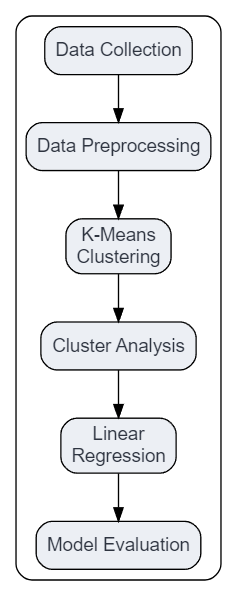
\includegraphics[width=\linewidth]{fig1.png}}
    \caption{Stages to determine the Risk Level of Pulmonary Tuberculosis.}
    \label{fig1}
\end{figure}

In this study, the authors aim to use advanced machine learning techniques to understand pulmonary tuberculosis (TB) epidemiology and guide prevention and control strategies. They plan to:
\begin{itemize}
    \item Implement K-Means clustering to identify TB risk patterns.
    \item Stratify individuals into risk groups based on demographics and clinical data.
    \item Apply linear regression to assess TB risk factors within each cluster.
    \item Evaluate model performance against traditional methods.
    \item Identify influential TB risk factors.
    \item Suggest targeted interventions for TB prevention and control.
\end{itemize}

\section{Related Works}
The reviewed paper provides a thorough examination of pulmonary tuberculosis (TB), detailing the lung as the primary infection site, symptoms, laboratory examinations, chest radiography, and CT scans. It discusses TB in the elderly, those on anti-tumor necrosis factor alpha inhibitors, and the diagnosis of pleural TB. The paper also covers pulmonary TB in HIV patients and its complications [1]. A significant portion addresses childhood pulmonary TB, highlighting three key concepts from chemotherapy literature: accurate case definitions, risk stratification, and the diverse spectrum of disease pathology. These concepts are crucial for diagnosing and treating childhood TB [2]. The paper compares risk factors for extra-pulmonary TB and pulmonary TB, emphasizing the global health burden of TB. It outlines diagnostic criteria based on various cultures and histological findings, defining extra-pulmonary TB per guidelines from the American Thoracic Society and the CDC [3]. Chemotherapy protocols for pulmonary TB are reviewed, noting the importance of continued treatment to prevent drug resistance. The efficacy of rifapentine and isoniazid in the continuation phase of treatment is critically evaluated, suggesting potential benefits of once-weekly dosing [4]. A case-control study in Samara, Russia identified key TB risk factors as raw milk consumption and unemployment. A study in Portugal linked TB risk to HIV/AIDS, prison population, unemployment, and overcrowded housing. Another study in Vitoria, Brazil highlighted the high risk of TB infection and disease among household contacts of TB patients [5]. Overall, the paper offers a comprehensive analysis of TB diagnosis, treatment, and risk factors, underlining the need for ongoing research and public health measures to combat TB globally.

\section{Methodology}
The stages of research methodology in applying clustering k-means and linear regression for determining the level of risk of pulmonary tuberculosis are as follows: 

\begin{figure}[H]
    \centerline{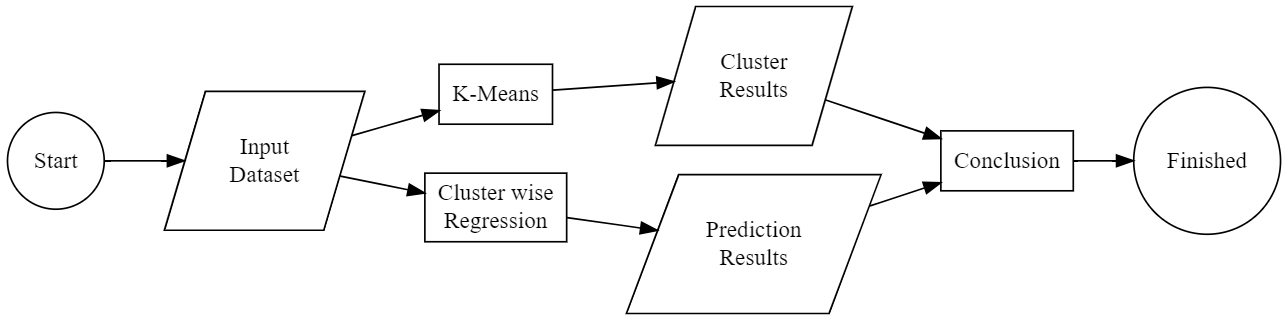
\includegraphics[width=\linewidth]{fig2.png}}
    \caption{Stages of Research Methodology for Determining Pulmonary TB.}
    \label{fig2}
\end{figure}

The collected tuberculosis dataset is divided into two groups using k-means clustering and linear regression.  The value of k will determine the number of clusters. The datasets in k-means show the cluster results.  Then cluster-wise Regression is the prediction results.  The combination of cluster results and prediction results is the final result.  Analyzing the data in this process is more effective in determining high-risk areas for pulmonary tuberculosis.

\subsection{Problem Identification and Data Processing}
Data analysis in machine learning involves two stages: clustering model with the K-Means algorithm and Cluster Regression method to determine clusters of high-risk pulmonary TB areas and forecasting models to examine the impact of population density on the number of pulmonary tuberculosis patients and to find solutions to the problems generated based on the results of the data sets entered in the analysis.

\subsection{Research Data Analysis}
Data analysis in classifying high-risk areas for pulmonary TB. The criterion data are variables used to determine high-risk areas for pulmonary tuberculosis. The research data are as follows:

\begin{table}[H]
    \centering
    \begin{tabular}{|c|c|c|c|c|c|}
    \hline
    \textbf{No} & \textbf{District} & \textbf{No} & \textbf{District} & \textbf{No} & \textbf{District} \\
    \hline
    1 & Dhaka & 7 & Gazipur & 13 & Mymensingh \\ \hline
    2 & Barisal & 8 & Jamalpur & 14 & Jessore \\ \hline
    3 & Khulna & 9 & Faridpur & 15 & Bogura \\ \hline
    4 & Rangpur & 10 & Chittagong & 16 & Tangail \\ \hline
    5 & Comilla & 11 & Sylhet & 17 & Dinajpur \\ \hline
    6 & Narayanganj & 12 & Rajshahi & & \\
    \hline
    \end{tabular}
    \caption{Research Data}
    \label{tab:research_data}
\end{table}
    

\subsubsection{K-Means Clustering Algorithm}
Data clustering is performed for each area by processing it into a cluster, and the k-means algorithm can determine cluster levels in each area based on the values of objects with different values in each group. The cluster model can also identify complex clustering values in determining high-risk areas for diseases. Furthermore, the k-means model can be divided into one or more clusters/groups. This method divides data into clusters or groups, grouping data with similar characteristics into the same cluster, and grouping data with different characteristics into other groups.
The analysis of the Clustering model with the K-Means algorithm in determining risk levels in clustering can divide data into clusters into several groups. Data mining models can group data with similar characteristics into the same cluster and group data with different characteristics into another group.

\begin{enumerate}
\item Determine the number of clusters to be formed.
\item Decide on random centroids and initialize clusters according to the number of clusters.
\item Calculate the distance to the centroid using the Euclidean Distance formula, as follows:

\[d = \sqrt{(x_2 - x_1)^2 + (y_2 - y_1)^2}
\]

This formula can be generalized to higher dimensions as well. In three-dimensional space, for example, with points \((x_1, y_1, z_1)\) and \((x_2, y_2, z_2)\), the Euclidean distance \(d\) is:


\[
    d = \sqrt{(x_2 - x_1)^2 + (y_2 - y_1)^2 + (z_2 - z_1)^2}
\]

And in n dimensions:

\[
    d = \sqrt{\sum_{i=1}^n (x_{2i} - x_{1i})^2}
\]

where \((x_{1i}, x_{2i})\) are the coordinates of the points in each dimension.
\item Observe the clustering data with the closest distance value to the centroid.
\item Determining the data center or new centroid.
\end{enumerate}

Next, Data analysis of the Linear regression model used in notation X and one response variable that can be represented by Y. Linear regression is used to assess the extent of influence between one variable and another.

\subsubsection{Cluster-wise Regression}
There are three methods for cluster-wise regression: linear regression, Finite Mixture Method (FMM), and cluster-weighted method (CWM). The linear regression method consists of one or more independent variables commonly denoted as X and one response variable represented by Y. Linear regression is used to obtain the forecast value with a variable related to another variable and can make better predictions. Therefore, it is preferable to implement a cluster initialization process using Cluster-wise Regression modeling in the next stage. One effective technique for cluster initialization is the Clustering method.


\subsection{Research Data}
The dataset for the study on the Application of K-Means Clustering and Linear Regression in Determining the Risk Level of Pulmonary Tuberculosis is as follows:

\begin{table}[H]
    \centering
    \begin{tabularx}{\linewidth}{|X|X|X|X|X|}
    \hline
    \textbf{Number} & \textbf{Area} & \textbf{Population (People)} & \textbf{Area (km²)} & \textbf{Pulmonary} \textbf{TB Cases} \\
    \hline
    1 & Dhaka & 23,936,000 & 369 & 1 \\ \hline
    2 & Barisal & 549,000 & 13.23 & 1 \\ \hline
    3 & Khulna & 965,483 & 59.57 & 0 \\ \hline
    4 & Rangpur & 445,677 & 2308 & 6 \\ \hline
    5 & Comilla & 670,775 & 153 & 3 \\ \hline
    6 & Narayanganj & 286330 & 33.57 & 5 \\ \hline
    7 & Gazipur & 213 061 & 49.32 & 3 \\ \hline
    8 & Jamalpur & 150 172 & 2031.98 & 11 \\ \hline
    9 & Faridpur & 122 425 & 66.24 & 19 \\ \hline
    10 & Chittagong & 5,513,609 & 5,282.98 & 13 \\ \hline
    11 & Sylhet & 999,374 & 26.5 & 0 \\ \hline
    12 & Rajshahi & 983,707 & 34,513 & 18 \\ \hline
    13 & Mymensingh & 497,562 & 91.32 & 2 \\ \hline
    14 & Jessore & 110 541 & 2610 & 0 \\ \hline
    15 & Bogra & 944,877 & 72.5 & 5 \\ \hline
    16 & Tangail & 180,144 & 29.04 & 7 \\ \hline
    17 & Dinajpur & 206,234 & 20.7 & 1 \\
    \hline
    \end{tabularx}
    \caption{Research Data Set}
    \label{tab:research_data_set}
    \end{table}

    \section{Results and Discussion}

    Research utilizing the K-Means algorithm for determining the risk levels of pulmonary tuberculosis (TB) has effectively divided data into distinct clusters. This analysis categorizes areas into different risk groups: two areas fall into the first cluster (low risk), several areas into the second cluster (moderate risk), and the remaining areas into the third cluster (high risk).
Following the clustering analysis, the study employs the Clusterwise Regression method to predict the impact of population density on the number of pulmonary TB cases. This approach assesses how population density influences the incidence of pulmonary TB across different areas, providing insights into the correlation between these variables and aiding in targeted public health interventions.
    
    \textbf{Application of the K-Means Algorithm Method}
    
    \subsection{Data on the population distribution of each sub district}
    The population distribution in the application of k-means clustering and linear regression in determining the risk level of pulmonary tuberculosis is as follows:
    
    \begin{table}[H]
        \centering
        \begin{tabularx}{\linewidth}{|X|X|X|X|X|}
        \hline
        No & District & Population (People) & Area (Km²) & Number of TB Patients \\
        \hline
        1 & Dhaka & 23,936,000 & 369 & 1 \\ \hline
        2 & Barisal & 549,000 & 13.23 & 1 \\ \hline
        3 & Khulna & 965,483 & 59.57 & 0 \\ \hline
        ... & ... & ... & ... & ... \\ \hline
        15 & Bogura & 944,877 & 72.5 & 5 \\ \hline
        16 & Tangail & 180,144 & 29.04 & 7 \\ \hline
        17 & Dinajpur & 206,234 & 20.7 & 1 \\
        \hline
        \end{tabularx}
        \caption{Data on the distribution of the number of pulmonary TB patients in each district}
        \label{tab:tb_data}
        \end{table}
    
    \subsection{Initialize the Cluster Center}
    
    The following table shows the population, area, and number of TB patients in each district, along with their assigned clusters after iteration:
    
    \begin{table}[h]
        \centering
        \begin{tabularx}{\linewidth}{|p{0.9cm}|p{1.75cm}|p{1.3cm}|p{0.7cm}|p{2cm}|}
        \hline
        \textbf{Iteration} & \textbf{Information} & \textbf{Population} & \textbf{Area (km²)} & \textbf{Number of Pulmonary TB} \\
        \hline
        Dhaka & Cluster1= C1 & 23,936,000 & 369 & 1 \\ \hline
        Barisal & Cluster 2 = C2 & 549,000 & 13.23 & 1 \\ \hline
        Khulna & Cluster 3 = C3 & 965,483 & 59.57 & 0 \\
        \hline
        \end{tabularx}
        \caption{Iteration Details}
        \label{tab:iteration_details}
    \end{table}
    
    \subsection{Nearest Cost Values Using Euclidean Distance}
    
    Euclidean Distance is a method used to determine the shortest path or minimum distance between two points in a multidimensional
space. In the context of clustering and the given table, the Euclidean Distance helps determine the nearest cluster for each data point 
based on their calculated cost. The nearest cost values are determined by calculating the Euclidean Distance. 
The results are as follows:   
    
\begin{table}[h]
    \centering
    \begin{tabularx}{\linewidth}{|X|X|X|X|X|}
    \hline
    C1 & C2 & C3 & Cluster Proximity & Cluster Assignment \\
    \hline
    0 & 23908700 & 23867051 & 0.0000 & C1 \\ \hline
    23908700 & 0 & 416483.83 & 0.0000 & C2 \\ \hline
    23867051.26 & 416483.0026 & 0 & 0.0000 & C3 \\ \hline
    5952.07231 & 2645.354067 & 17979.00106 & 2645.3541 & C2 \\ \hline
    4164.530169 & 868.3768975 & 19771.00014 & 868.3769 & C2 \\ \hline
    ... & ... & ... & ... & ... \\ \hline
    24150.14635 & 27457.17456 & 48081.03475 & 24150.1464 & C1 \\ \hline
    16433.14822 & 13126.26785 & 7498.120815 & 7498.1208 & C3 \\ \hline
    8848.596239 & 5542.23089 & 15083.18804 & 5542.2309 & C2 \\
    \hline
    \multicolumn{4}{|r|}{Total Proximity} & 98672.3064 \\
    \hline
    \end{tabularx}
    \caption{Table 5. Distance (Cost) Values in the First Iteration}
    \label{tab:distance_values}
\end{table}


\subsection{Information}
\begin{itemize}
    \item \textbf{Distance of Dhaka to Clusters} \\
    $D_1(c_1) = \\ \sqrt{(239636000 - 239636000)^2 + (369 - 369)^2 + (1 - 1)^2} \\ = 0$ \\
    $D_1(c_2) = \\ \sqrt{(239636000 - 549000)^2 + (369 - 13.23)^2 + (1 - 1)^2} \\ = 239087000$ \\
    $D_1(c_3) = \\ \sqrt{(239636000 - 965483)^2 + (369 - 59.57)^2 + (1 - 0)^2} \\ = 238670517$

    \item \textbf{Distance of Barisal to Clusters} \\
    $D_2(c_1) = \\ \sqrt{(549000 - 239636000)^2 + (13.23 - 369)^2 + (1 - 1)^2} \\ = 239087000$ \\
    $D_2(c_2) = \\ \sqrt{(549000 - 549000)^2 + (13.23 - 13.23)^2 + (1 - 1)^2} \\ = 0$ \\
    $D_2(c_3) = \\ \sqrt{(549000 - 965483)^2 + (13.23 - 59.57)^2 + (1 - 0)^2} \\ = 416483.0026$

    \item \textbf{Distance of Khulna to Clusters} \\
    $D_3(c_1) = \\ \sqrt{(965483 - 239636000)^2 + (59.57 - 369)^2 + (0 - 1)^2} \\ = 238670517$ \\
    $D_3(c_2) = \\ \sqrt{(965483 - 549000)^2 + (59.57 - 13.23)^2 + (0 - 1)^2} \\ = 416483.83$ \\
    $D_3(c_3) = \\ \sqrt{(965483 - 965483)^2 + (59.57 - 59.57)^2 + (0 - 1)^2} \\ = 0$ 
\end{itemize}

Each row in the table shows the distance of a point from each cluster center (C1, C2, C3). The "Cluster Proximity" column shows the smallest distance, and the "Nearest Cluster" column indicates the corresponding cluster assignment based on this minimum distance.
\begin{itemize}
    \item Selection of the Fourth Centroid
    \item Results of the Fourth Iteration Process
\end{itemize}



The cluster centers (centroids) remain unchanged in this iteration. The new centroids obtained from the previous iteration are used to calculate the distances using Euclidean distance. The results are as follows:

\begin{table}[h]
\centering
\begin{tabularx}{\linewidth}{|X|X|X|X|}
\hline
\textbf{Cluster} & \textbf{Population (people)} & \textbf{Area (km²)} & \textbf{Number of TB Patients} \\ \hline
Cluster 1 (C1) & 55617.5 & 37.995 & 18.5 \\ \hline
Cluster 2 (C2) & 19646.33333 & 105.1 & 3.444444444 \\ \hline
Cluster 3 (C3) & 30597.16667 & 129.3933333 & 5.333333333 \\ \hline
\end{tabularx}
\caption{Final Centroid Centers for the Fourth Iteration}
\label{tab:my_label}
\end{table}

These centroids represent the centers of the clusters after the fourth iteration, calculated based on the population, area, and number of TB patients. The Euclidean distance is used to determine the proximity of each district to these centroids.

\subsection{Results of the Fourth Iteration}
The calculations for the fourth iteration of applying machine learning clustering using k-means and linear regression for determining the risk level are as follows:

The results in Table 7 represent the completion of the iteration process for the third centroid. Then, the fourth iteration was carried out using the new centroids.

\begin{table}[H]
    \centering
    \begin{tabular}{|p{.1cm}|p{1.1cm}|p{.7cm}|p{0.50cm}|p{0.85cm}|p{0.85cm}|p{1cm}|p{0.4cm}|}
    \hline
    \textbf{No} & \textbf{Population} & \textbf{Area (km²)} & \textbf{No. of TB Patients} & \textbf{Cluster 1} & \textbf{Cluster 2} & \textbf{Cluster 3} & \textbf{Clu- ster Gr- oup} \\ \hline
    12 & 983707 & 34513 & 18 & 1704.63 & 37675.69 & 42895.36 & C1 \\ \hline
    8 & 150172 & 203198 & 11 & 16410.66 & 19560.67 & 24780.32 & C1 \\ \hline
    9 & 122425 & 6624 & 19 & 1704.63 & 34266.78 & 23316.17 & C2 \\ \hline
    3 & 965483 & 5957 & 0 & 46376.57 & 10405.34 & 5185.74 & C2 \\ \hline
    5 & 670775 & 153 & 3 & 43113.60 & 7142.37 & 1923.08 & C2 \\ \hline
    13 & 497562 & 91.32 & 2 & 39703.54 & 3732.35 & 1487.30 & C2 \\ \hline
    14 & 110541 & 2610 & 0 & 42924.57 & 6953.34 & 1733.85 & C2 \\ \hline
    .. & ... & ... & ... & ... & ... & ... & .. \\ \hline
    .. & ... & ... & ... & ... & ... & ... & .. \\ \hline
    1 & 23,936,000 & 369 & 1 & 22445.75 & 13525.72 & 18745.46 & C3 \\ \hline
    2 & 549,000 & 13.23 & 1 & 25752.77 & 10218.79 & 15438.41 & C3 \\ \hline
    4 & 445,677 & 2308 & 6 & 28397.60 & 7573.67 & 12793.34 & C3 \\ \hline
    6 & 286330 & 33.57 & 5 & 26607.92 & 9366.97 & 14586.03 & C3 \\ \hline
    16 & 180,144 & 29.04 & 7 & 30465.50 & 5505.97 & 10725.79 & C3 \\ \hline
    17 & 206,234 & 20.7 & 1 & 31293.50 & 4678.14 & 9897.47 & C3 \\ \hline
    \end{tabular}
    \caption{Results of the Fourth Iteration}
    \label{tab:my_label2}
    \end{table}

     The result of this process shows that there are differences in the cluster numbers for each area based on the new centroid values. In the fourth iteration, the cluster results did not change, meaning that the third and fourth clusters remained the same, and the iteration process was stopped. Therefore, it can be concluded that:

    \begin{itemize}
        \item 2 regions are included in Cluster 1
        \item 6 regions are included in Cluster 2
        \item 9 regions are included in Cluster 3
    \end{itemize}

    \subsection{Results of the K-Means Clustering Algorithm}
    \subsubsection{Cluster Results with K-Means Using Python}
    The cluster results for each sub-district, distributed across each region using the k-means algorithm, are as follows:

    \begin{table}[H]
        \centering
        \begin{tabular}{|c|c|c|c|}
        \hline
        \textbf{Sub-District} & \textbf{Cluster\_km} & \textbf{Sub-District} & \textbf{Cluster\_km} \\ \hline
        Dhaka & 2 & Narayanganj & 2 \\ \hline
        Barisal & 2 & Gazipur & 2 \\ \hline
        Khulna & 1 & Jamalpur & 2 \\ \hline
        Rangpur & 2 & Faridpur & 0 \\ \hline
        Comilla & 1 & Chittagong & 1 \\ \hline
        Sylhet & 2 & Rajshahi & 0 \\ \hline
        Mymensingh & 1 & Jessore & 1 \\ \hline
        Bogra & 1 & Tangail & 2 \\ \hline
        Dinajpur & 2 & & \\ \hline
        \end{tabular}    
        \caption{K-Means Cluster Results}
        \label{tab:my_label3}
    \end{table}
    

    \subsubsection{K-Means Cluster Graph Results}
    The graphical representation of the implementation of K-Means Clustering and Linear Regression in determining the risk level of pulmonary tuberculosis is as follows:

    \begin{figure}[H]
        \centerline{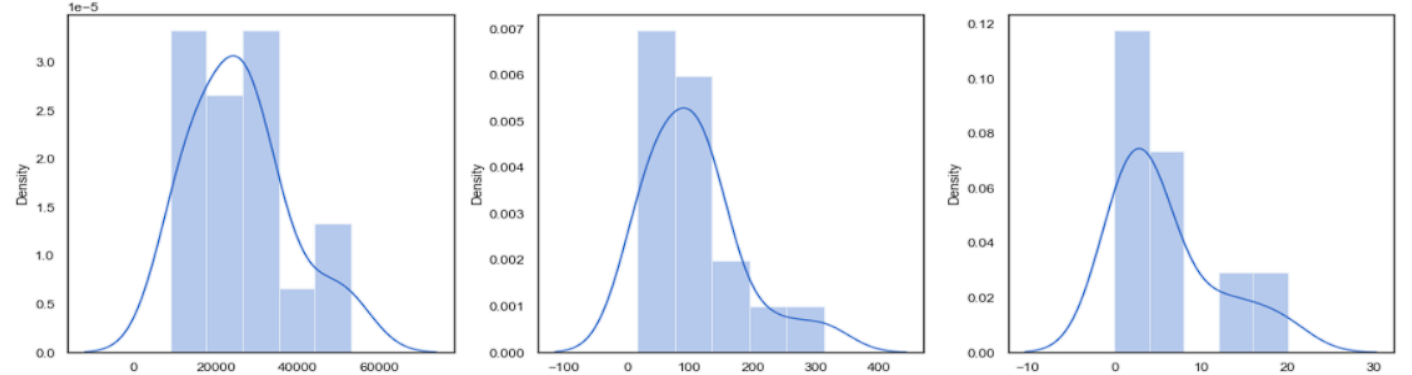
\includegraphics[width=\linewidth]{fig3.png}}
        \caption{K-Means Cluster Graph.}
        \label{fig3}
    \end{figure}

    \subsection{Linear Regression Algorithm}
\subsubsection{Results of $X^2$, $Y^2$ and $XY$}
The results for the values of $X^2$, $Y^2$, and $XY$ to find the total are as follows:

\begin{table}[H]
    \centering
    \begin{tabular}{|c|c|c|c|c|c|}
    \hline
    \textbf{No} & \textbf{X} & \textbf{Y} & \textbf{$X^2$} & \textbf{$Y^2$} & \textbf{$XY$} \\ \hline
    1 & 235 & 1 & 55225 & 1 & 235 \\ \hline
    2 & 192 & 1 & 36864 & 1 & 192 \\ \hline
    3 & 81 & 0 & 6561 & 0 & 0 \\ \hline
    4 & 242 & 6 & 58564 & 36 & 1452 \\ \hline
    5 & 98 & 3 & 9604 & 9 & 294 \\ \hline
    6 & 93 & 5 & 8649 & 25 & 465 \\ \hline
    7 & 151 & 3 & 22801 & 9 & 453 \\ \hline
    8 & 359 & 11 & 128881 & 121 & 3949 \\ \hline
    .. & .. & .. & .. & .. & ..\\ \hline
    .. & .. & .. & .. & .. & ..\\ \hline
    15 & 233 & 5 & 54289 & 25 & 1165\\ \hline
    16 & 536 & 7 & 287296 & 49 & 3752\\ \hline
    17 & 629 & 11 & 395641 & 121 & 6919 \\ \hline
    Total & 9251 & 100 & 14182549 & 1160 & 109865 \\ \hline
    \end{tabular}
    \caption{Table 9. Results for $X^2$, $Y^2$, and $XY$}
    \label{tab:my_label4}
\end{table}

This table shows the calculated values for $X^2$, $Y^2$, and $XY$, which are used in the linear regression analysis to determine the relationship between the variables $X$ and $Y$. The totals at the bottom are the sums of each column.

\subsubsection{Calculation of the Model Coefficients $a$ and $b$}

To calculate the coefficients $a$ (the intercept) and $b$ (the slope) in the linear regression model $Y=a+bX$, we use the following formulas:

Slope ($b$):\\



    $b = \frac{n \left( \sum XY \right) - \left( \sum X \right) \left( \sum Y \right)}{n \left( \sum X^2 \right) - \left( \sum X \right)^2} = 2.58415$

    \textbf{Intercept (a)}

$$a = \frac{\left( \sum Y \right) \left( \sum X^2 \right) - \left( \sum X \right) \left( \sum XY \right)}{n \left( \sum X^2 \right) - \left( \sum X \right)^2}= 0.00606$$
$$r^2 = \frac{b \left( \sum XY \right)}{\sum Y^2} = 0.57403$$

Y= 2.58415 + 0.00606X\\
Given the totals from Table 9:
\begin{itemize}
    \item $\sum X = 9251$
    \item $\sum Y = 100$
    \item $\sum X^2 = 14182549$
    \item $\sum Y^2 = 1160$
    \item $\sum XY = 109865$
    \item $n = 17$ (number of observations)
\end{itemize}

This means that approximately 57\% of the variation in the dependent variable (x), which is population density, can explain the variation in the number of pulmonary tuberculosis patients. In other words, the variable (x) has an influence of 57\% on the variable (y).

\subsection{Calculating the Linear Regression Model Equation}
The simple linear regression equation is given by: \\ $Y=a+bX$. Using the calculated coefficients $a=2.584154827$ and $b=0.006060898$, we can predict the values of $Y$ for given values of $X$.

\subsubsection{Calculation of Predicted Values}


For $X=235$: \\
$Y=2.584154827+0.006060898 \times 235 = 2.584154827+1.424311044 = 4.008465871$

For $X=192$:\\
$Y=2.584154827+0.006060898 \times 192 = 2.584154827+1.163692428 = 3.747847255$

For $X=242$:\\
$Y=2.584154827+0.006060898 \times 242 = 2.584154827+1.46673733 = 4.050892157$

For $X=98$:\\
$Y=2.584154827+0.006060898 \times 98 = 2.584154827+0.594268004 = 3.178422831$

For $X=93$: \\
$Y=2.584154827+0.006060898 \times 93 = 2.584154827+0.563664614 = 3.147819441$

For $X=151$:\\
$Y=2.584154827+0.006060898 \times 151 = 2.584154827+0.915195898 = 3.499350725$

For $X=359$: \\
$Y=2.584154827+0.006060898 \times 359 = 2.584154827+2.176055794 = 4.760210621$

For $X=1138$: \\
$Y=2.584154827+0.006060898 \times 1138 = 2.584154827+6.89730199 = 9.481456817$

By applying the regression formula, we can predict the number of tuberculosis patients based on the given population densities.

\subsection{Graph of the Influence of Population Density on the Number of Pulmonary TB Patients}

The graph depicting the influence of population density on the number of pulmonary tuberculosis patients is as follows:

\begin{figure}[H]
    \centerline{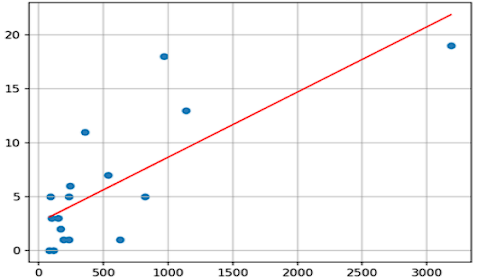
\includegraphics[width=\linewidth]{fig4.png}}
    \caption{Influence of Population Density on the Number of Pulmonary TB Patients.}
    \label{fig4}
\end{figure}


\section{Conclusion}
The analysis using the K-means algorithm identified specific areas susceptible to pulmonary tuberculosis, guiding targeted interventions. Clustering revealed three clusters, enabling tailored strategies for each. Cluster-wise Regression showed population density explains 57\% of TB variation, highlighting demographic factors' importance. However, other variables contribute to the remaining variation, warranting further exploration for comprehensive interventions. This combined approach offers a powerful framework for understanding disease patterns and informing interventions. Yet, limitations like data quality and narrow variables exist. Future research should integrate diverse data sources and employ non-linear modeling for enhanced understanding and more effective tuberculosis control strategies.

\begin{thebibliography}{00}
\bibitem{b1} B. Ula Mutammimul, Bakhtiar, Desvina Yulisda, Badriana, “Application Of The Fuzzy Time Series Model In Clothing Material Stock Forecasting,” J. Sist. Inf. Dan Ilmu Komput. Prima (JUSIKOM PRIMA), vol. 6, no. 1, pp. 56-61, 2022, doi: https://doi.org/10.34012/jurnalsisteminformasidanilmukomputer.v6i1.286 2.
\bibitem{b2} CLUSTER-WISE REGRESSION PADA STATISTICAL DOWNSCALING UNTUK PENDUGAAN CURAH HUJAN BULANAN,” Indones. J. Stat. Its Appl., vol. 3, no. 3, pp. 236-246, Oct. 2019, doi: 10.29244/IJSA.V3I3.310.
\bibitem{b3} F. Hardiyanti, H. S. Tambunan, and I. S. Saragih, “PENERAPAN METODE K- MEDOIDS CLUSTERING PADA PENANGANAN KASUS DIARE DI INDONESIA,” KOMIK (Konferensi Nas. Teknol. Inf. dan Komputer), vol. 3, no. 1, Dec. 2019, doi: 10.30865/komik.v3i1.1666.
\bibitem{b4} G. Gustientiedina, M. H. Adiya, and Y. Desnelita, “Penerapan Algoritma K- Means Untuk Clustering Data Obat-Obatan,” J. Nas. Teknol. dan Sist. Inf., vol. 5, no. 1, pp. 17–24, Apr. 2019, doi: 10.25077/TEKNOSI.V5I1.2019.17-24.
\bibitem{b5} Gustientiedina Gustientiedina, M. Hasmil Adiya, and Yenny Desnelita, “Penerapan Algoritma K-Means Untuk Clustering Data Obat-Obatan,” J. Nas. Teknol. dan Sist. Inf., vol. 5, no. 1, pp. 17-24, Apr. 2019, doi: 10.25077/TEKNOSI.V5I1.2019.17-24.
\bibitem{b6} M. U. Fitria, Rahma, Desvina Yulisda, “Data Mining Classification Algorithms For Diabetes Dataset Using Weka Tool,” J. Sist. Inf., vol. 2, no. 1, 2021.
\bibitem{b7} M. Ula, A. F. Ulva, Mauliza, M. A. Ali, and Y. R. Said, “Application Of Machine Learning In Predicting Children's Nutritional Status With Multiple Linear Regression Models,” MULTICA Sci. Technol. J., vol. 2, no. 2, pp. 124–130, Feb. 2022, doi: 10.47002/MST.V2I2.363.
\bibitem{b8} N. Puspitasari, N. Puspitasari, and F. Urmila Jannah Helmi Puadi, “Klasterisasi Wilayah Penghasil Tanaman Lada Menggunakan Algoritma K- Means,” Indones. J. Comput. Sci., vol. 11, no. 3, Dec. 2022, Accessed: Feb. 20, 2023.	[Online].	Available:
\bibitem{b9} R. A. Rizal, N. O. Purba, L. A. Siregar, K. Sinaga, and N. Azizah, “Analysis of Tuberculosis (TB) on X-ray Image Using SURF Feature Extraction and the K- Nearest Neighbor (KNN) Classification Method,” JAICT, vol. 5, no. 2, pp. 9–12, Oct. 2020, doi: 10.32497/JAICT.V5I2.1979.

	
\end{thebibliography}


\end{document}
